\documentclass[a4paper,11pt]{article}
\usepackage{tabularx}
\usepackage{geometry}
\usepackage{xcolor}
\usepackage{physics}
\usepackage[most]{tcolorbox}
\usepackage{amsmath}
\usepackage{amssymb}
\usepackage{multicol}
\usepackage{float}
\usepackage{graphicx}
\usepackage{fancybox}
\usepackage{caption}
\usepackage{amsthm}
\usepackage{url}

\tcbuselibrary{breakable}
\geometry{left=1.4cm, top=0.8cm, right=1.2cm, bottom=1cm}

% Entorno para ejercicios con recuadro azul
\newtcolorbox{ejercicio}[1]{
    colback=white!8, colframe=blue!5!black,
    boxrule=0.75pt, arc=5pt, boxsep=10pt,
    title={\textbf{Ejercicio #1}}, fonttitle=\bfseries,
    breakable,
    before upper={\parindent15pt} % Añade sangría al texto
}

% Entorno para demostraciones con recuadro verde
\newtcolorbox{demostracion}[1]{
    colback=blue!5, colframe=gray!50!black,
    boxrule=0.75pt, arc=5pt, boxsep=10pt,
    title={\textbf{#1}}, fonttitle=\bfseries,
    breakable
}

\providecommand{\abs}[1]{\ensuremath{\left|#1\right|}}
\providecommand{\paren}[1]{\ensuremath{\left(#1\right)}}
\providecommand{\corche}[1]{\ensuremath{\left[#1\right]}}
\newcommand{\E}[1]{\mathbb{E}\left[#1\right]} % Esperanza
\newcommand{\LG}[1]{\mathcal{L}\left[#1\right]} % Transformada de Laplace
\newcommand{\LGV}[1]{\mathbb{L}\left[#1\right]} %
\newcommand{\V}[1]{\mathbb{V}\left[#1\right]} % Varianza
\newcommand{\COV}[2]{\mathbb{COV}\left[#1, #2\right]} % Covarianza
\NewDocumentCommand{\VA}{m}{\mathbf{#1}}

%----------HEADING-----------------
\begin{document}

\begin{tcolorbox}[colback=gray!10, colframe=black, boxrule=0.5pt, arc=5pt, boxsep=5pt]
\begin{tabularx}{\linewidth}{X r}
  \begin{tabular}[t]{@{}l@{}}
    \textbf{Introducción a la Ciencia de Datos} \\
    \textbf{Tarea I}
  \end{tabular}
  &\textbf{Antonio Barragán}\\
  &\textbf{Hazel Sánchez}\\
   & \textbf{Omar García Ramos} \\
\end{tabularx}
\end{tcolorbox}


%======================== DESCRIPCION DE LA BASE DE DATOS ====================

\section{Descripción de la base de datos}

El conjunto de datos está organizado en un \texttt{DataFrame} con \textbf{415 observaciones} (filas) y \textbf{26 variables} (columnas).
Contiene información sobre sitios de muestreo de árboles en Europa y sus registros isotópicos ($\delta^{13}C$) a lo largo de varios años.
Los valores faltantes se indican como \texttt{NA}.

\subsection*{Estructura de las variables}

Estadisticas basicas
\begin{table}[ht]
    \centering
    \caption{Estadísticas descriptivas de los datos}
    \label{tab:estadisticas_basicas}
    \begin{tabular}{|l|c|c|c|c|}
        \hline
        & count & unique & top & freq \\
        \hline
        Site Code & 415 & 415 & Site  name & 1 \\
        BRO & 111 & 38 & -25,5 & 10 \\
        CAV  & 374 & 39 & -24,2 & 38 \\
        CAZ  & 412 & 41 & -20,7 & 35 \\
        COL    & 289 & 31 & -21,0 & 37 \\
        DRA  & 235 & 50 & -23,8 & 18 \\
        FON  & 292 & 148 & -24,20 & 7 \\
        GUT  & 412 & 193 & -23,07 & 6 \\
        ILO & 412 & 45 & -23,4 & 36 \\
        INA  & 412 & 40 & -24,7 & 34 \\
        AHI & 293 & 53 & -24,3 & 21 \\
        LAI  & 201 & 45 & -25,5 & 13 \\
        LIL & 408 & 47 & -21,9 & 23 \\
        LOC  & 264 & 41 & -26,6 & 21 \\
        NIE1 & 413 & 258 & NA  & 27 \\
        NIE2 & 413 & 50 & -23,1 & 32 \\
        PAN  & 412 & 118 & NA  & 216 \\
        PED  & 410 & 187 & -21,77 & 6 \\
        POE  & 412 & 55 & -23,4 & 24 \\
        REN  & 376 & 235 & -25,34 & 5 \\
        SER & 409 & 46 & -22,0 & 34 \\
        SUW  & 414 & 49 & -23,3 & 22 \\
        VIG  & 337 & 40 & -23,2 & 30 \\
        VIN  & 159 & 46 & -22,4 & 15 \\
        WIN & 244 & 40 & -23,1 & 21 \\
        WOB  & 408 & 54 & -25,6 & 27 \\
        \hline
    \end{tabular}
\end{table}

%===============================================================================

\begin{table}[ht]
    \centering
    \caption{Tipos de datos, valores no nulos y faltantes por columna}
    \label{tab:info_datos}
    \begin{tabular}{|l|c|c|c|c|}
        \hline
        Columna & Tipo & No nulos & Valores faltantes & Porcentaje faltante \\
        \hline
        Site Code & object & 415 & 0 & 0.000000 \\
        BRO & object & 111 & 304 & 73.253012 \\
        CAV  & object & 374 & 41 & 9.879518 \\
        CAZ  & object & 412 & 3 & 0.722892 \\
        COL    & object & 289 & 126 & 30.361446 \\
        DRA  & object & 235 & 180 & 43.373494 \\
        FON  & object & 292 & 123 & 29.638554 \\
        GUT  & object & 412 & 3 & 0.722892 \\
        ILO & object & 412 & 3 & 0.722892 \\
        INA  & object & 412 & 3 & 0.722892 \\
        AHI & object & 293 & 122 & 29.397590 \\
        LAI  & object & 201 & 214 & 51.566265 \\
        LIL & object & 408 & 7 & 1.686747 \\
        LOC  & object & 264 & 151 & 36.385542 \\
        NIE1 & object & 413 & 2 & 0.481928 \\
        NIE2 & object & 413 & 2 & 0.481928 \\
        PAN  & object & 412 & 3 & 0.722892 \\
        PED  & object & 410 & 5 & 1.204819 \\
        POE  & object & 412 & 3 & 0.722892 \\
        REN  & object & 376 & 39 & 9.397590 \\
        SER & object & 409 & 6 & 1.445783 \\
        SUW  & object & 414 & 1 & 0.240964 \\
        VIG  & object & 337 & 78 & 18.795181 \\
        VIN  & object & 159 & 256 & 61.686747 \\
        WIN & object & 244 & 171 & 41.204819 \\
        WOB  & object & 408 & 7 & 1.686747 \\
        \hline
    \end{tabular}
\end{table}




\subsection*{Valores Faltantes}

Mostramos una grafica de como se distribuyen los datos faltantes en la tabla. Cada casilla en blanco indica que es un valor faltante (NaN).

\begin{figure}[ht]
	\centering
	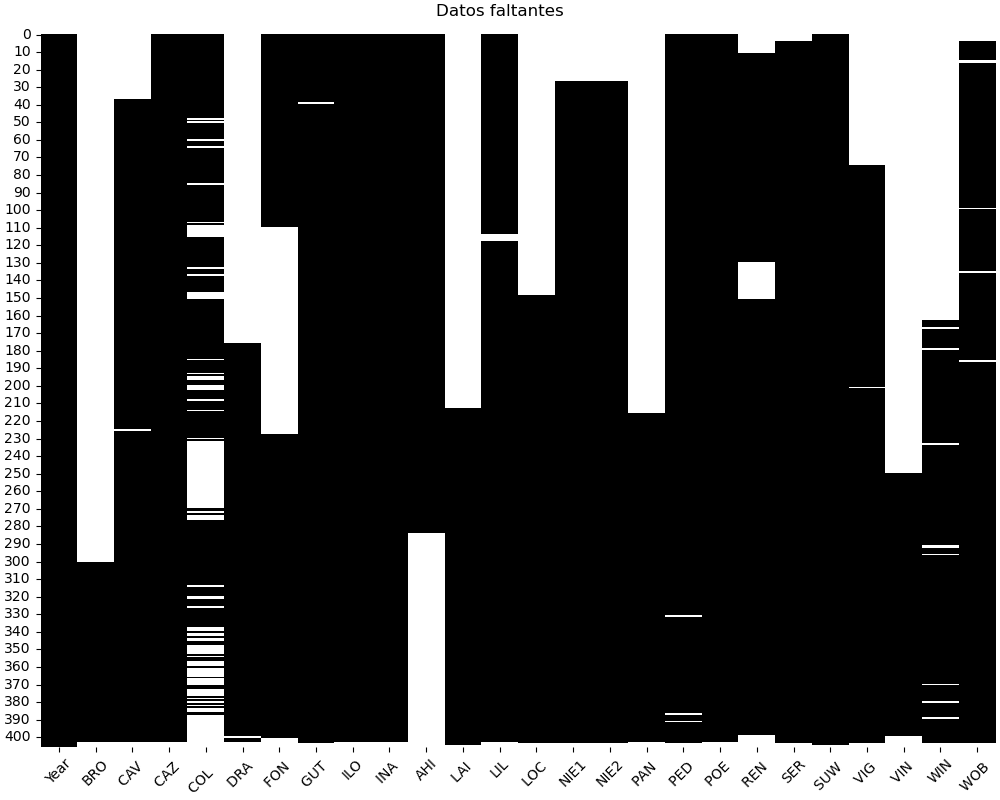
\includegraphics[width=0.7\linewidth]{figures/faltantes}
	\caption{Mapa de color - Datos faltantes}
	\label{fig:faltantes}
\end{figure}

En la grafica podemos identificar patrones que sugieren que la medición de los datos en ciertas variables falló de manera continua por ciertos periodos, mientras que en otras variables los datos faltantes parecen seguir otra distribución, y finalmente encontramos variables en las cuales los datos faltantes son muy pocos o ninguno.


\subsection*{Clasificación de las variables según su escala de medición}

A continuación se presenta la clasificación de cada variable de la base de datos según su escala de medición. Se incluye una breve explicación del porqué de cada clasificación.

\begin{itemize}
    \item \textbf{Site Code}: Nominal.
    Se trata de un identificador de los sitios de muestreo, por lo que no posee un orden ni valor numérico significativo.

    \item \textbf{BRO}: Razón ($\delta$13C).
    Representa valores isotópicos medidos, donde el cero tiene un significado absoluto y las diferencias entre valores son significativas.

    \item Continuara...

\end{itemize}

\end{document}